\section{Results}

\subsection{Calibration and verification: parameter spin-up}

 %Write in the results that the innovations for eta and pi show that the model can reproduce observed supply elasticities and crop production 


The model parameters were spun-up to equilibrium with the conditions of 2008 (first year of the analysis period) by ingesting observations from that year during 20 assimilation cycles. The results of the parameter spin-up showed that for most counties the parameters could be accurately inferred from the assimilated observations. An example for Beaverhead county (a county with a large extent of land allocated to agriculture and also first county alphabetically) is shown in Figure \ref{fig:calibration_spinup}. Results for all counties are presented in online Appendix A. The ensemble was initiated before the spin-up with an arbitrary mean and a large spread (initial coefficient of variation of the ensemble was prescribed at 300\%) and the ensembles typically converged to a steady state distribution with very low variance within five to eight assimilation cycles. The quick convergence of the mean and the variance indicates that the observations contained sufficient information to identify the model parameters values.  Figure \ref{fig:innovation_spinup} show the dynamics of the ensemble of innovations (residual between Eq. \eqref{eq:LHS} and Eq. \eqref{eq:RHS}) for the parameter evolution of Beaverhead county shown in Figure \ref{fig:calibration_spinup}. The figure shows that, in general, the innovation quickly approached zero, which indicates that the convergence of the parameter ensembles was to a solution that satisfied the optimality conditions of the positive mathematical program (Eq. \eqref{eq:optimality_program}). The algorithm works because components (1) and (2) in Eq. \eqref{eq:LHS} represent the marginal revenues with respect to land and water allocation, and components (1) and (2) of Eq. \eqref{eq:RHS} represent the respective marginal costs. When the ensemble of differences between $LHS_i$ and $RHS_i$ is centered about zero the methodology is effectively solving the first order conditions of the net revenue maximization problem, which is the core of the calibration algorithm. Although the innovation component associated with most equations showed quick convergence, some of them, such as component (2) of the innovation for irrigated spring wheat or for irrigated alfalfa in Beaverhead county, converged to a nonzero value. Biases in component (2) of the innovation indicate that the parameter ensemble of $\lambda_{water}$ converged to a suboptimal value. Online Appendix B shows the evolution of the innovation ensembles associated with the parameter spin-ups in all counties in the state of Montana.    

\begin{figure}
\includegraphics[width=0.8\textwidth]{Figures/cal_spin_Beaverhead.pdf}
\label{fig:calibration_spinup}
\caption{Evolution of the parameter ensemble during parameter spin-up in Beaverhead county. Shaded areas are the 95 and 68 percentile confidence intervals of the ensemble. Ensembles for all counties is presented in online Appendix A}
\end{figure}


\begin{table}[]
\resizebox{0.8\textwidth}{!}{%
\centering
\begin{threeparttable}
\caption{Mean relative bias (Rel. Bias \tnote{a}) and relative root mean square error (Rel. RMSE\tnote{b}) statistics for the simulation land allocated during the 2008 benchmark conditions. }
\label{tab:gof_spinup}

\begin{tabular}{|l|l|l|l|l|}
\hline
                          & \multicolumn{4}{c|}{2018}                                                         \\ \hline
                          & \multicolumn{2}{c|}{Land Use}           & \multicolumn{2}{c|}{Water Use}          \\ \hline
                          & \textit{Rel. Bias} & \textit{Rel. RMSE} & \textit{Rel. Bias} & \textit{Rel. RMSE} \\ \hline
Alfalfa Irrigated         & -0.062             & 0.142              & -0.172             & 0.257              \\ \hline
Alfalfa Nonirrigated      & -0.021             & 0.08              & -                  & -                  \\ \hline
Barley Irrigated          & 1.826              & 1.939             & 2.694208           & 1.125              \\ \hline
Barley Nonirrigated       & -0.020             & 0.018              & -                  & -                  \\ \hline
Spring Wheat Irrigated    & -0.028             & 0.138              & 0.715453           & 1.00               \\ \hline
Spring Wheat Nonirrigated & -0.020             & 0.014              & -                  & -                  \\ \hline
Winter Wheat              & -0.019             & 0.062              & -                  & -                  \\ \hline
\end{tabular}%

\begin{tablenotes}\footnotesize
\item [a] $Rel. Bias = \frac{sim_i - obs_i}{obs_i}$
\item [b] $Rel. RMSE = \frac{\sqrt{\frac{1}{n}\sum_i^n(sim_i - obs_i)^2}}{\frac{1}{n}\sum_i^n obs_i}$
\end{tablenotes}
\end{threeparttable}
}
\end{table}


The ensemble of parameters obtained at the end of the spin-up cycle was used to predict the land and water allocation for the 2008 baseline. Although the ensemble of innovations indicate that some parameter distributions converge to suboptimal values, the model was able predict land and water allocations with satisfactory accuracy, as summarized in Table \ref{tab:gof_spinup}. The correlation coefficient between county-wise simulated and observed land allocation is higher than 0.98 and the relative bias of the estimation is typically less than 0.06 (6\%). The exception are the simulation of land allocated to irrigated barley, which showed significantly lower correlation and higher bias than the other crops.         

\begin{figure}
\includegraphics[width=0.8\textwidth]{Figures/inn_spin_Beaverhead.pdf}
\label{fig:innovation_spinup}
\caption{Evolution of the filter innovation during parameter spinup corresponding to the ensembles in Figure \ref{fig:calibration_spinup}. Subscript of column titles refer to a innovation component as numbered in Eqs. \eqref{eq:LHS} and \eqref{eq:RHS}. Shaded areas are the 95 and 68 percentile confidence intervals of the ensemble. Ensemble for all counties is presented in online Appendix B}
\end{figure}

A comparison between the predicted probability distributions of land and water allocation and actual allocations provides a direct evaluation of the model predictive skills for individual counties and also illustrates how parameter uncertainty translates into uncertainty in the predictions of resource allocation. Figure \ref{fig:hist_land_alloc} shows the simulated probability distribution of land allocated to the crops grown in Beaverhead county along with the observed allocation. Online appendix C shows the simulated land allocation for all crops and counties. In general, for most counties and crops, the predictive distributions are well centered around the observation or bracket the observations within the high probability density interval. The probability distribution of the predictions reflect the sensitivity of predictions to the spread of the parameter ensemble.  

\begin{figure}
\includegraphics[width=0.8\textwidth]{Figures/30001_hist_2008.png}
\label{fig:hist_land_alloc}
\caption{Simulated probability distributions (blue bars) and observed (red lines) land allocation in 2009 for seven crops grown in Beaverhead county, MT. Simulations for all counties is presented in online Appendix C.}
\end{figure}

Comparison between observed and modeled water allocation for irrigation is less straightforward because water allocation per crop and county is not directly observed. Remote sensing ET observations only provide total crop water use, which integrates water from natural precipitation and from supplemental irrigation. However, the simulation scenarios require that the the expected amount of water from natural sources used by crops (natural ET) is specified.  However, the simulation scenarios require that the the expected amount of water from natural sources used by crops (natural ET) is specified. Subtracting this specified natural ET amount from the total observed crop water use gives us an estimate of the amount of crop water use supplemented by irrigation. This estimate served as the observation of supplemental irrigation used to evaluate the model simulation of water allocation.  Figure \ref{fig:hist_water_alloc} shows the case of Beaverhead county. Figures for water allocation in all counties in the state are provided in online appendix D. Similar to the simulation of land use, the simulation of water allocation per crop and county is also centered around the observations, bracketing them in most cases within the high probability region of predictions.   

\begin{figure}
\includegraphics[width=0.6\textwidth]{Figures/30001obs_water_hist_2008.png}
\label{fig:hist_water_alloc}
\caption{Simulated probability distribution of water allocation for three irrigated crops grown in Beaverhead county, MT (blue bars). Dashed grey vertical line indicates the observed total evapotranspiration consumed by the crop (evaporation from natural supplies and from supplemental irrigation). Benchmark supplemental irrigation (red vertical line), was estimated by subtracting water used by crops from natural supplies  (natural ET) as prescribed in the modeled scenario from the observed total crop evapotranspiration. Simulations for all counties is presented in online Appendix D.}
\end{figure}

\subsection{Dynamics of the parameter ensemble}

Using the parameter distributions obtained at the end of the spin-up period as a starting point, we assimilated remote sensing observations from 2009 through 2016. Figure \ref{fig:calibration2008-2015} shows the dynamics of the parameter ensembles for Beaverhead county over the the eight years of data assimilation. Note that the $y$ axis has been re-scaled with respect to that of Figure \ref{fig:calibration_spinup} to better represent the ensemble spread. Figures for all counties are available in online appendix E. In general, parameters $\beta_{land}$ and $\beta_{water}$ showed very high stability and very little dispersion over time, with very small drifts in their mean value. To a lesser degree, parameter $\delta$ also presented relatively high stability and low ensemble dispersion. On the other hand, $\lambda_{land}$, $\lambda_{water}$, and the $\mu$ parameters showed large ensemble dispersion and high sensitivity to variations in the input observations. The evolution of the parameters sometimes exhibited smooth drifts over the data assimilation period (e.g. parameter $\mu$ for non-irrigated spring wheat non-irrigated in Figure \ref{fig:calibration2008-2015}), sudden realignments after a specific year (e.g. the case of $\lambda_{land}$, $\lambda_{water}$ for winter wheat and $\overline{\lambda}_{fsl}$ in year 2010), or fluctuations about a long term mean without a clear trend (e.g. parameter $\mu$ for winter wheat in Figure \ref{fig:calibration2008-2015})).


\begin{figure}
\includegraphics[width=0.8\textwidth]{Figures/cal_Beaverhead.pdf}
\label{fig:calibration2008-2015}
\caption{Dynamics of the parameter ensembles over 8 years (2008-2016) of data assimilation in Beaverhead county. Parameters start from the distribution achieved at the end of the spin-up period in 2008. Shaded areas are the 95 and 68 percentile confidence intervals of the ensemble. Figures for all other counties are presented in Online Appendix E. }
\end{figure}

The dynamics of the innovation associated with the parameter ensembles in Fig.\ref{fig:calibration2008-2015} were in general tightly centered around zero for most components, reflecting the precision and accuracy with which the parameters can be tracked over time (Figure \ref{fig:innovation20082015}). The filter maintained most of the parameters at optimal values and indicated that the model was ready for operational use throughout the assimilation period. The exception to this was component (2) of the innovation, which showed high variance and a significant bias for alfalfa and irrigated winter wheat. Although Figure \ref{fig:innovation20082015} represents the case of Beaverhead county, component (2) of the innovation was often the one that exhibited the largest amount of bias and variance over all counties. This component of the innovation is controlled by parameter $\lambda_{water_i}$, which was shown in Fig. \ref{fig:calibration2008-2015} to be the least identifiable parameter.  

%The evolution of the parameters is required to meet the optimality conditions embedded in the filter, however the equation that describes the artificial evolution of the parameters (Eq. \eqref{eq:param_evolution}) contains a smoothing factor that controls the sensitivity of the parameter ensemble to new information. Damping the response of the parameters to observations makes their dynamics more stable but also can generate suboptimal innovations.




\subsection{Simulation of years 2017 and 2018}

Table \ref{tab:gof} shows the relative bias and root mean square relative error (RMSRE) of the mean predicted vs observed crop acreage and water allocation over all counties in Montana for years 2017 and 2018. For these simulations, the model was run with the parameter distribution obtained at the end of the 2008-2016 assimilation period. For most crops, the simulation of the 2017 land and water use showed a higher bias and RMSRE than in 2018. This larger model predictive error in 2017 is associated with the abnormal conditions generated by the severe flash drought that affected the US Northern Plains in the summer of 2017 \citep{He2019, Kimball2019}.  Despite the better predictive performance of the model in 2018, the results for the two simulated years are qualitatively very similar and therefore we only present and discuss the predictions for year 2017. The discussion of the results from 2017 also apply to the simulations of year 2018.        

\begin{figure}
\includegraphics[width=0.8\textwidth]{Figures/figure_Beaverhead.pdf}
\label{fig:innovation20082015}
\caption{Dynamic of the innovation over 8 years (2008-2015) of assimilation corresponding to the parameter ensembles shown in Figure \ref{fig:calibration_spinup}. Subscript of column titles refer to a innovation component as numbered in Eqs. \eqref{eq:LHS} and \eqref{eq:RHS}. Shaded areas are the 95 and 68 percentile confidence intervals of the ensemble. Ensemble for all counties is presented in online Appendix F}
\end{figure}

% Please add the following required packages to your document preamble:
% \usepackage{graphicx}
\begin{table}[]
\resizebox{0.8\textwidth}{!}{%
\centering
\begin{threeparttable}
\caption{Mean relative bias (Rel. Bias \tnote{b}) and relative root mean square error (Rel. RMSE \tnote{b}) statistic for the simulation of land allocation and water allocation under the conditions of years 2017 and 2018.}
\label{tab:gof}

\begin{tabular}{|l|l|l|l|l|l|l|l|l|}
\hline
                          & \multicolumn{4}{c|}{2017}                                      & \multicolumn{4}{c|}{2018}                                      \\ \hline
                          & \multicolumn{2}{c|}{Land use} & \multicolumn{2}{c|}{Water use} & \multicolumn{2}{c|}{Land use} & \multicolumn{2}{c|}{Water use} \\ \hline
 &
  \textit{Rel. Bias} &
  \textit{Rel. RMSE} &
  \textit{Rel. Bias} &
  \textit{Rel. RMSE} &
  \textit{Rel. Bias} &
  \textit{Rel. RMSE} &
  \textit{Rel. Bias} &
  \textit{Rel. RMSE} \\ \hline
Alfalfa Irrigated         & -0.003         & 0.151        & -0.172         & 0.805         & -0.067         & 0.182        & -0.104         & 0.542         \\ \hline
Alfalfa Nonirrigated      & 0.155          & 0.277        & -              & -             & -0.045         & 0.133        & -              & -             \\ \hline
Barley Irrigated          & 0.319          & 0.305        & 2.694          & 3.09          & -0.193         & 0.379        & 5.745          & 3.135         \\ \hline
Barley Nonirrigated       & 0.301          & 0.476        & -              & -             & -0.155         & 0.226        & -              & -             \\ \hline
Spring Wheat Irrigated    & 1.321          & 0.540        & 0.715          & 2.511         & 2.531          & 0.508        & 0.419          & 2.05          \\ \hline
Spring Wheat Nonirrigated & -0.005         & 0.285        & -              & -             & -0.037         & 0.165        & -              & -             \\ \hline
Winter Wheat              & -0.241         & 0.488        & -              & -             & -0.167         & 0.089        & -              & -             \\ \hline
\end{tabular}%
\begin{tablenotes}\footnotesize
\item [a] $Rel. Bias = \frac{sim_i - obs_i}{obs_i}$
\item [b] $Rel. RMSE = \frac{\sqrt{\frac{1}{n}\sum_i^n(sim_i - obs_i)^2}}{\frac{1}{n}\sum_i^n obs_i}$
\end{tablenotes}
\end{threeparttable}
}
\end{table}

The model satisfactorily reproduced the county-scale distribution of cropping patterns (Figure \ref{fig:map_land_change}). Alfalfa is grown in all states and the model predictions capture well the spatial distribution of land allocation for this crop (Figure \ref{fig:map_land_change} rows 1 and 2). Note that the area planted with non-irrigated alfalfa tends to be larger in the eastern third of the state because that region is characterized by large properties and extensive ranching. This distribution is well captured in the model predictions. On the other hand, irrigated alfalfa is more common in the southern and southwest portions of the state, in counties close to the border with Wyoming and in the upstream end of the Gallatin, Yellowstone and Missouri rivers. This is also correctly captured by the model. Also remarkable is the ability of the model to identify the regions in the state that specialize in small grain production. The model correctly identifies the counties in the west and north west central region of Montana that allocate the most land to irrigated and non-irrigated barley (Figure \ref{fig:map_land_change} rows 3 and 4). It also identifies very well the swath of counties in the north and north east portions of the state that allocate the most land to grow spring wheat and winter wheat (Figure \ref{fig:map_land_change} rows 5 and 6). The spatial distribution of relative errors show some complex spatial patterns, but in general relative errors in simulated area allocated to a crop are largest in counties where observations of area planted with a given crop are small because relative errors are normalized by these observations. This causes the summary statistics presented in Table \ref{tab:gof} to be skewed by very large errors in a small number of counties. This is particularly evident in the statistics of land allocated to irrigated barley and irrigated spring wheat, where simulated land allocation tends to underestimate observations (negative relative errors represented by blue colors in Figure \ref{fig:map_land_change}), but Table \ref{tab:gof} reports a large positive relative bias.     
 
\begin{figure}
\includegraphics[width=\textwidth]{Figures/mean_land_use_2018.png}
\label{fig:map_land_change}
\caption{Comparison between model simulated (left column) and observed (center column) land allocated in 2017 to the major crops grown in Montana.  Right panel shows the relative prediction error defined as $\frac{simulated - observed}{observed}$. Counties with small amounts of observed land allocated to a given crop can produce disproportionately large relative errors. For visualization purposes, the error scale has been clipped to values from -1 to 1..}
\end{figure}

% \begin{figure}[t]
% \includegraphics[width=\textwidth]{Figures/248_streamflow_diversion.png}
% \label{fig:ts_q_div}
% \caption{[WARNING: PLACEHOLDER FIGURE]Expected change in water allocation the 2012 drought as a percentage of the 2009 baseline allocation for three selected irrigated crops.}
% \end{figure}


 The extent of land allocated to irrigated crops is, of course, an indication of the agricultural water demands. In general, agricultural water use is higher in counties that are closer to the river headwaters. Counties in the headwaters of the Missouri river and upstream tributaries (Jefferson, Madison and Gallatin Rivers, see Figure \ref{fig:hydro_network}), in the southwestern quadrant of the state, as well as counties in the upper course of the Yellowstone river in south central Montana, have some of the highest agricultural water consumption in the state, putting a significant amount of strain on the water supplies. This agricultural water consumption pattern is clearly represented in the simulated total agricultural applications per county (Figure \ref{fig:total_water_map}). The model underestimated the total agricultural water use in all counties (negative relative errors), however the relative underestimations are in general modest. Large relative errors in the predictions often occur in counties with relatively low observed supplemental irrigation.    

\begin{figure}
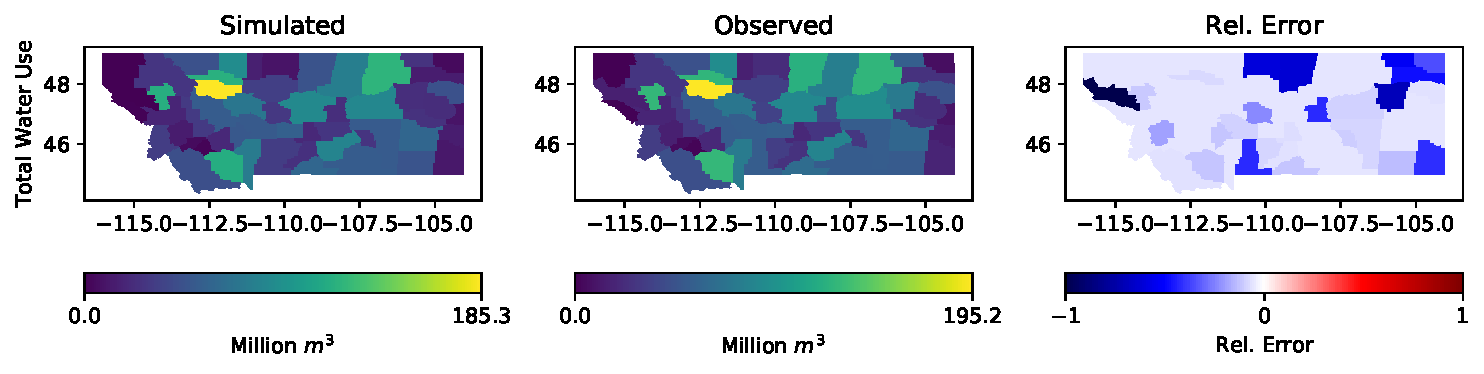
\includegraphics[width=0.9\textwidth]{Figures/total_water_use.pdf}
\label{fig:total_water_map}
\caption{Comparison between simulated (left panel) and observed (center panel) total agricultural water applications per county for year 2017. Right panel shows the relative prediction error defined as $\frac{simulated - observed}{observed}$. Counties with small amounts of observed irrigation can produce disproportionately large relative errors. For visualization purposes, the error scale has been clipped to values from -1 to 1. }
\end{figure}

Counties with high agricultural water use are expected to have the largest impacts on the hydrologic system. A strength of hydro-economic model is that it tracks the hydrologic impacts of agricultural activity. The spatial and temporal net effects of agricultural diversions on streamflows are shown in Figure \ref{fig:map_water_change}. Insets in Figure \ref{fig:map_water_change}a show simulated streamflows with and without the effects of water diversions for year 2017 in four nodes of the river network and the simulated water diversion rates from these nodes during the growing season. The standard profile of water diversion rates in all nodes followed the water demands associated with the progression of crops during the growing season. Water withdrawals start on the prescribed planting date of each crop, which for most crops is around May 15, increase as crops grow to full coverage, and finally taper down as crops mature before the prescribed harvesting date in late August. The impacts of water withdrawals on streamflows starts during the spring freshet, when streamflows are high, but it is typically maximal in late June or early August during low summer flows. When water diversions decline at the end of the summer, the model simulates the recovery of streamflows. 

\begin{figure}
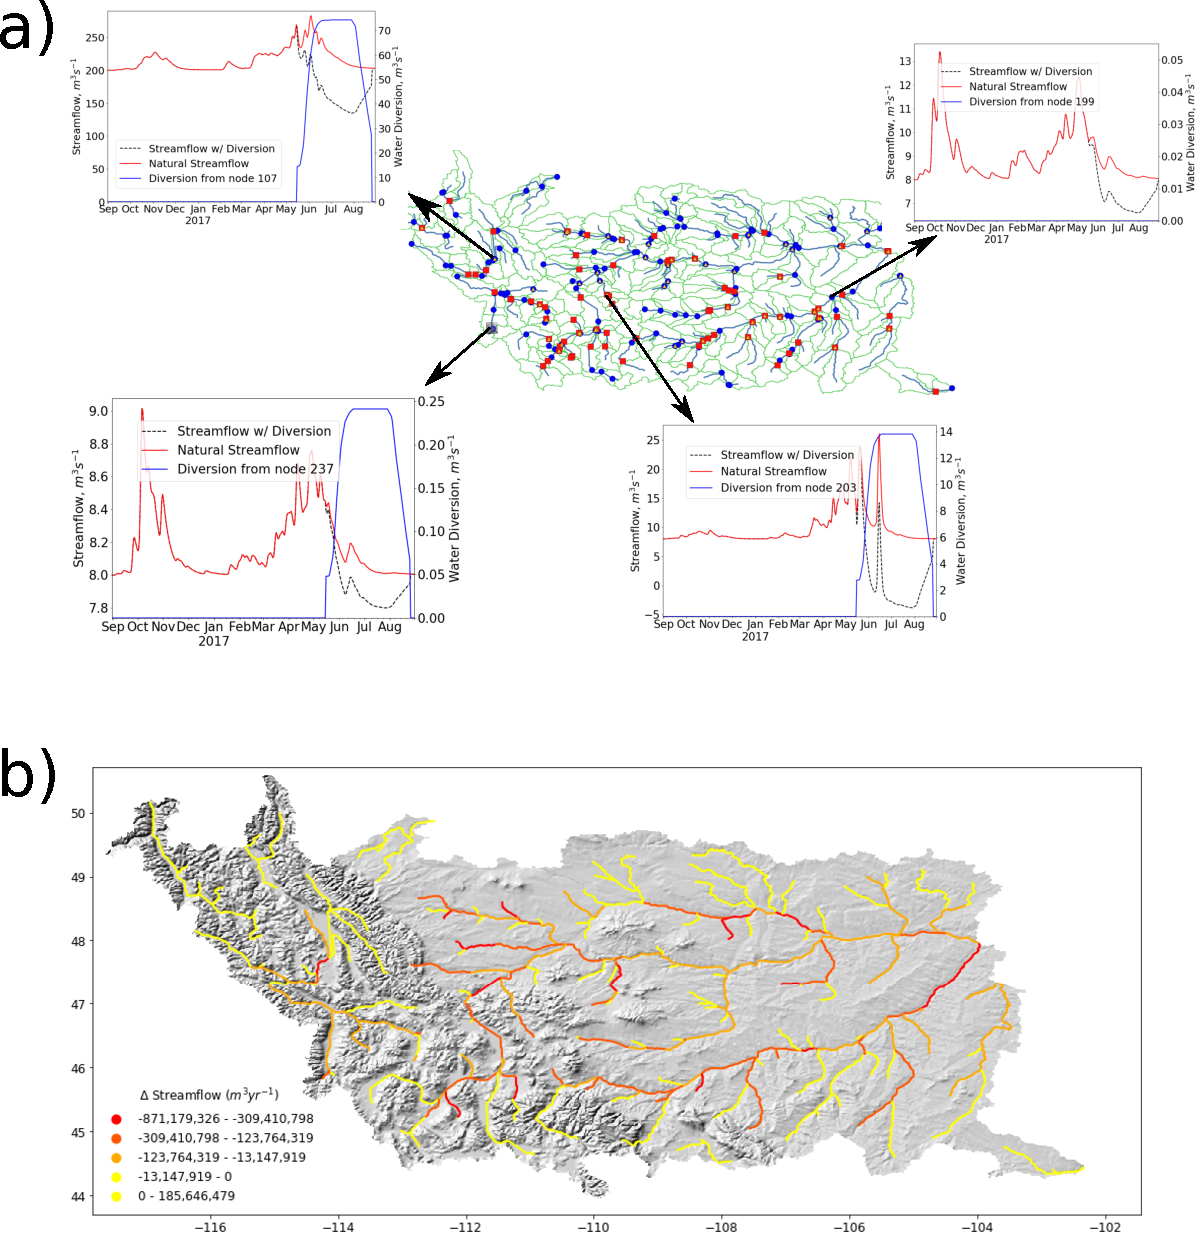
\includegraphics[width=\textwidth]{Figures/FigureWaterUse.pdf}
\label{fig:map_water_change}
\caption{Simulated hydrologic conditions during the 2016-2017 water year. Insets in a) show  time series of simulated streamflows assuming no agriculture (red line), simulated streamflows with diversions (black dotted line), and agricultural water diversion (blue line) for four nodes in the river network. Panel b) shows the spatial impacts of agriculture on total annual streamflow volumes. $Delta$ Streamflow is the difference in total annual simulated streamflow volumes between the no agriculture reference model and the model with active agricultural diversions.}
\end{figure}

The spatially distributed nature of the hydrologic model naturally simulates the downstream impacts of agricultural activity. For instance, the inset associated with the easternmost node in Figure \ref{fig:map_water_change}a is not a diversion node, so there are no agricultural water withdrawals from this location, however water diverted upstream still reduces the natural flows in late spring and summer. To appreciate better the spatial extent of streamflow drawdowns, we produced a visualization of the total net impact of agriculture on the hydrologic network in 2017 (Figure \ref{fig:map_water_change}b). The net impact ($\Delta$ Streamflow) was produced by calculating the total annual water volume difference between natural flows and flows under agricultural withdrawals. Unsurprisingly, the most impacted river reaches are those that supply water to counties with high agricultural water applications, such as those in the headwaters of the Missouri river (c.f. Figure \ref{fig:total_water_map}), however the impact of water diversion often extends far downstream, affecting counties where agricultural water demands are low. 